\subsection{Saturated Model Parameters ($\theta_{\sat}$) \label{sec::sat_est}}

\subsubsection{Bounding Condition}

From~(\ref{eqn::eta_sat}), $\bar\eta_{F,\sat}(k) = \phi_2^T(k)\,\theta_{\sat}$. Converting back to $\eta$ space, the
saturation ceiling bounds the actual $\nox$ reduction at every time step:
\begin{align}
    \eta_{\sat}(k) = \phi_{\sat}^T(k)\,\theta_{\sat} \geq \eta(k) \qquad \forall\, k
    \label{eqn::eta_sat_bound}
\end{align}
where $\phi_{\sat}(k) = \frac{u_1(k)}{F(k)}\,\phi_2(T(k))$ is the saturated-model regressor. This holds because a
fully saturated catalyst ($\sigma = \Gamma$) always produces at least as much reduction as any $\sigma \leq \Gamma$.
The bound is independent of the operating mode, so all data can be used without knowing when the catalyst is saturated.

\subsubsection{Linear Programming Formulation}

Since the bound must hold for every time step, the optimal $\hat\theta_{\sat}$ is the one that produces the tightest
possible envelope over the data. This is a linear program:
\begin{align}
    \hat\theta_{\sat} = \argmin_{\theta_{\sat}} \;\pmb{1}^T\,\Phi_{\sat}\,\theta_{\sat}
        \qquad \text{s.t.} \quad \Phi_{\sat}\,\theta_{\sat} \succeq H
    \label{eqn::sat_lp}
\end{align}
where $\Phi_{\sat} = \lrb{\phi_{\sat}(1), \ldots, \phi_{\sat}(N{-}1)}^T$ and
$H = \lrb{\eta(2), \ldots, \eta(N)}^T$.

The operating temperature range is partitioned into two zones to capture the non-monotone dependence of
$k_{scr}\,\Gamma$ on $T$. Each zone has its own $\theta_{\sat}$.

% --- Bounded eta figure ---
\begin{figure}[!ht]
    \begin{minipage}{0.49\textwidth}
        \centering
        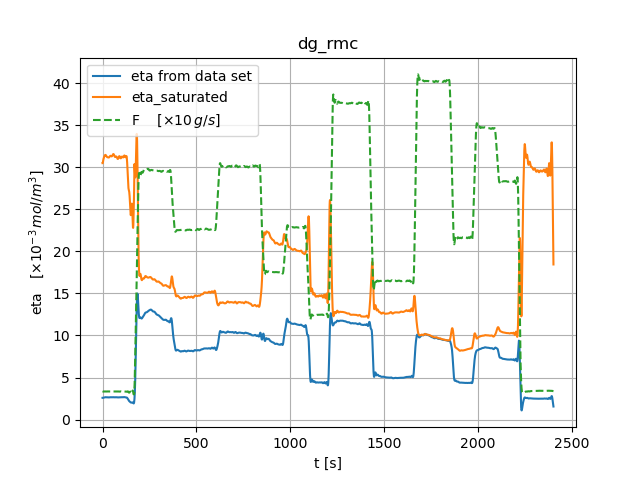
\includegraphics[width=\textwidth]{./figs/3-sysID/eta_bounds_dg_rmc.png}
    \end{minipage}
    \begin{minipage}{0.49\textwidth}
        \centering
        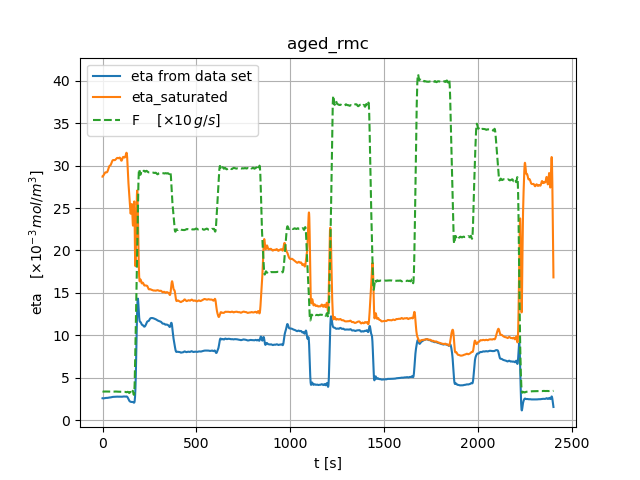
\includegraphics[width=\textwidth]{./figs/3-sysID/eta_bounds_aged_rmc.png}
    \end{minipage}
    \caption{Saturated ceiling (tight upper bound) for RMC data: degreened (left) and aged (right)}
    \label{fig::eta_bounds_rmc}
\end{figure}

\begin{figure}[!ht]
    \begin{minipage}{0.49\textwidth}
        \centering
        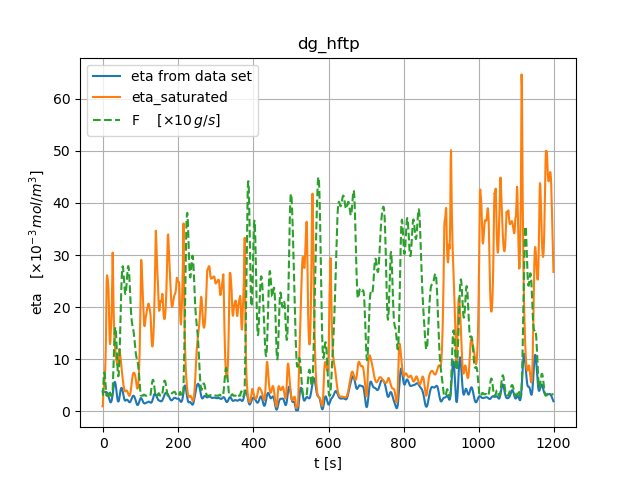
\includegraphics[width=\textwidth]{./figs/3-sysID/eta_bounds_dg_hftp.png}
    \end{minipage}
    \begin{minipage}{0.49\textwidth}
        \centering
        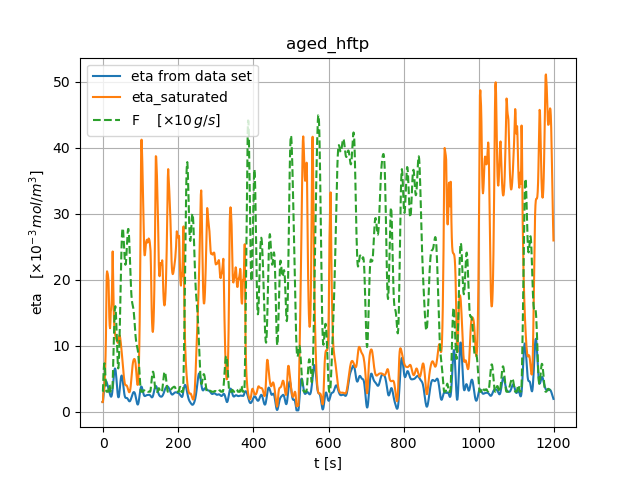
\includegraphics[width=\textwidth]{./figs/3-sysID/eta_bounds_aged_hftp.png}
    \end{minipage}
    \caption{Saturated ceiling for hot-FTP data: degreened (left) and aged (right)}
    \label{fig::eta_bounds_hftp}
\end{figure}

% --- Parameter table ---
\begin{table}[!ht]
    \centering
    \caption{$\theta_{\sat}$ estimates ($\theta_{\sat}[i]$: coefficient of $T^i$)}
    \label{tab::sat_parm_est}
    \begin{tabular}{l l r r r}
        \hline \hline
        \multicolumn{5}{c}{\textit{Degreened}} \\
        \hline
        Test & Zone & $[2]$ & $[1]$ & $[0]$ \\
        \hline
        RMC      & high & $-0.06$ & $1.43$ & $31.19$ \\
        hot-FTP  & high & $-0.49$ & $2.94$ & $40.94$ \\
        cold-FTP & high & $-0.19$ & $0.97$ & $40.69$ \\
        cold-FTP & low  & $0.26$  & $5.97$ & $45.00$ \\
        \hline
        \multicolumn{5}{c}{\textit{Aged}} \\
        \hline
        RMC      & high & $-0.07$ & $1.77$ & $27.82$ \\
        hot-FTP  & high & $-0.54$ & $3.40$ & $39.59$ \\
        cold-FTP & high & $-0.28$ & $1.82$ & $38.97$ \\
        cold-FTP & low  & $0.39$  & $8.25$ & $50.63$ \\
        \hline \hline
    \end{tabular}
\end{table}
